\section{Multi GPU Experiments}
\label{chap:results:sec:multi}

In the second part of our evaluation, we examine the performance of multi-GPU inference. We evaluate three multi-GPU nodes featuring 8 NVIDIA A100, 4 NVIDIA H100, and 8 AMD MI300x, respectively.
Each node is tested with three configurations, corresponding to tensor parallel sizes of 1, 2, and 4, and a data parallel size set to fully utilize the node's resources.
Using bfloat16 precision, we evaluate 10 models, while with FP8 quantization, we evaluate 14 LLMs.

The data is presented through two heatmaps (\ref{fig:heatmapbf16} and \ref{fig:heatmapfp8}), structured to have one row per model and three columns per node, corresponding to the different partitions.
The models are sorted by parameter count, while the columns correspond to different models and their TP/DP settings. Throughput is normalized by the number of data parallel instances, while energy efficiency does not need to be normalized due to weak scaling (see \ref{chap:methods:sec:multi}).

This data allows us to observe different trends of multi-GPU inference, including
(1) the scaling efficiency of Data and Tensor Parallelism,
(2) the impact of model size scaling on performance,
(3) a cross-vendor comparison of the three nodes, in a multi-GPU setting.

\begin{figure}[H]
    \centering
    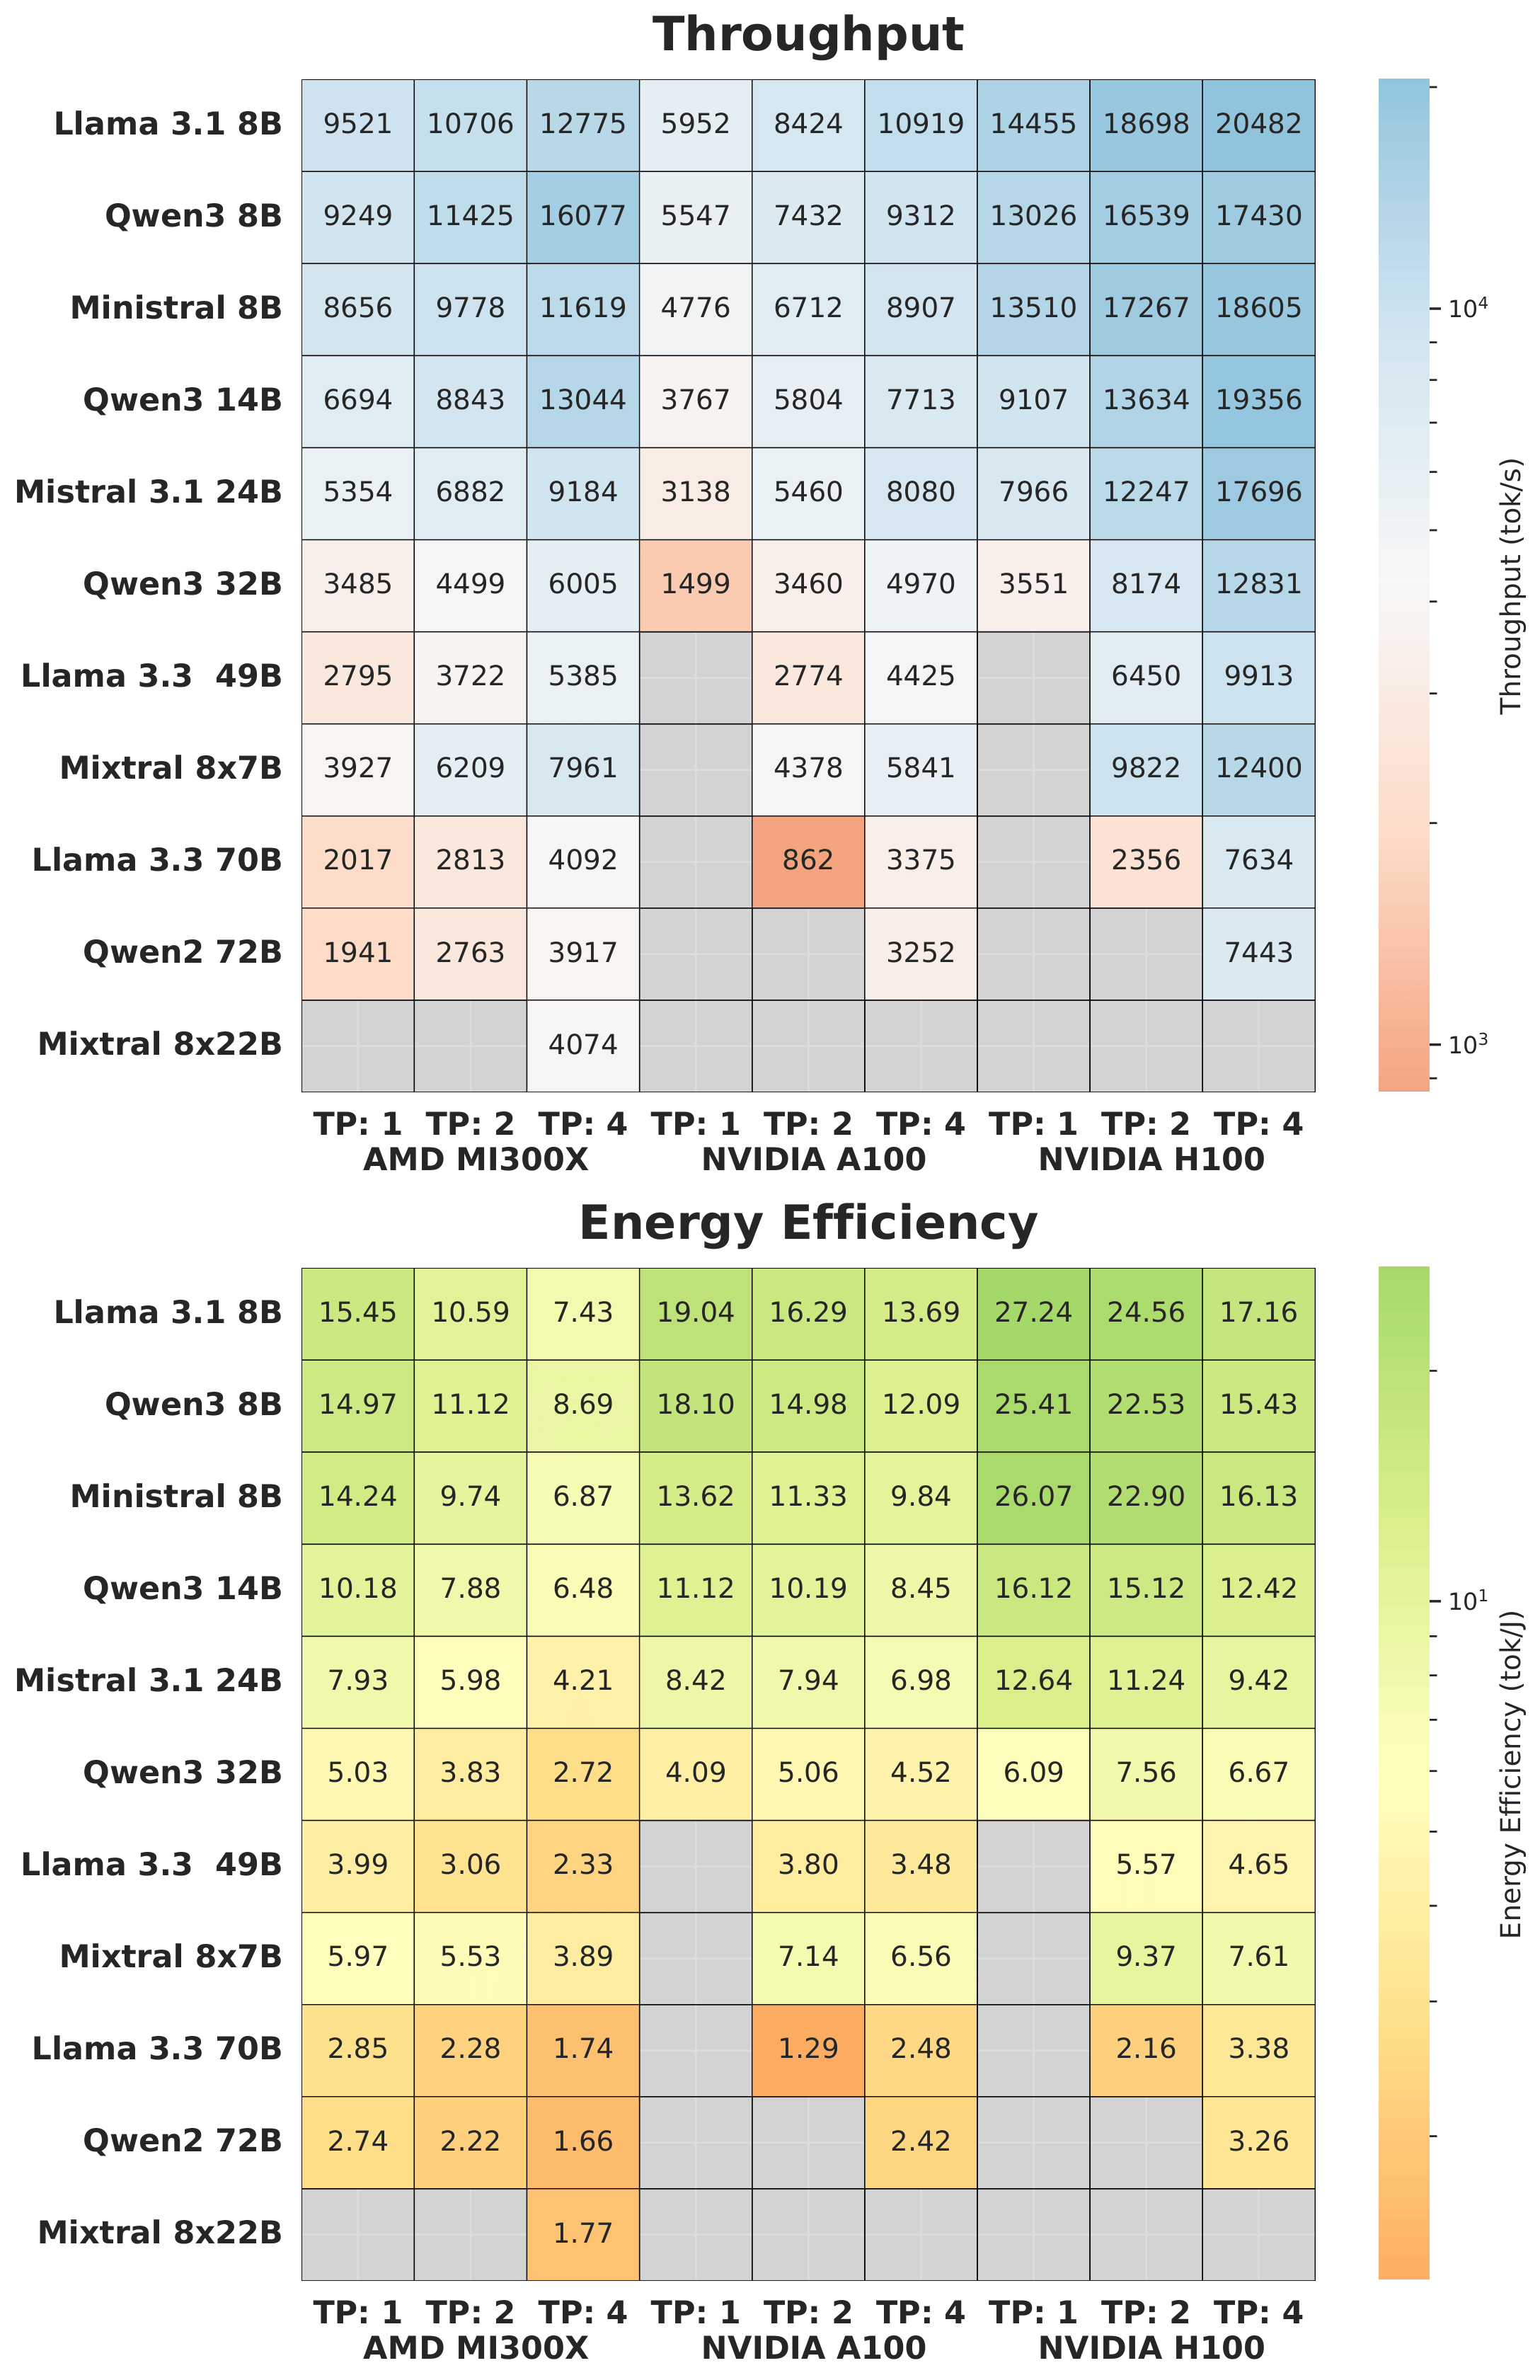
\includegraphics[width=0.9\columnwidth]{figs/heatmap Throughput (toks)_vs_Energy Efficiency (tokJ)_bfloat16.png}
    \caption{Throughput and energy efficiency heatmap across three multi-GPU nodes (bfloat16).}
    \tagpdfsetup{alttext={Throughput and energy efficiency heatmap across three multi-GPU nodes (bfloat16).}}
    \label{fig:heatmapbf16}
\end{figure}

\begin{figure}[H]
    \centering
    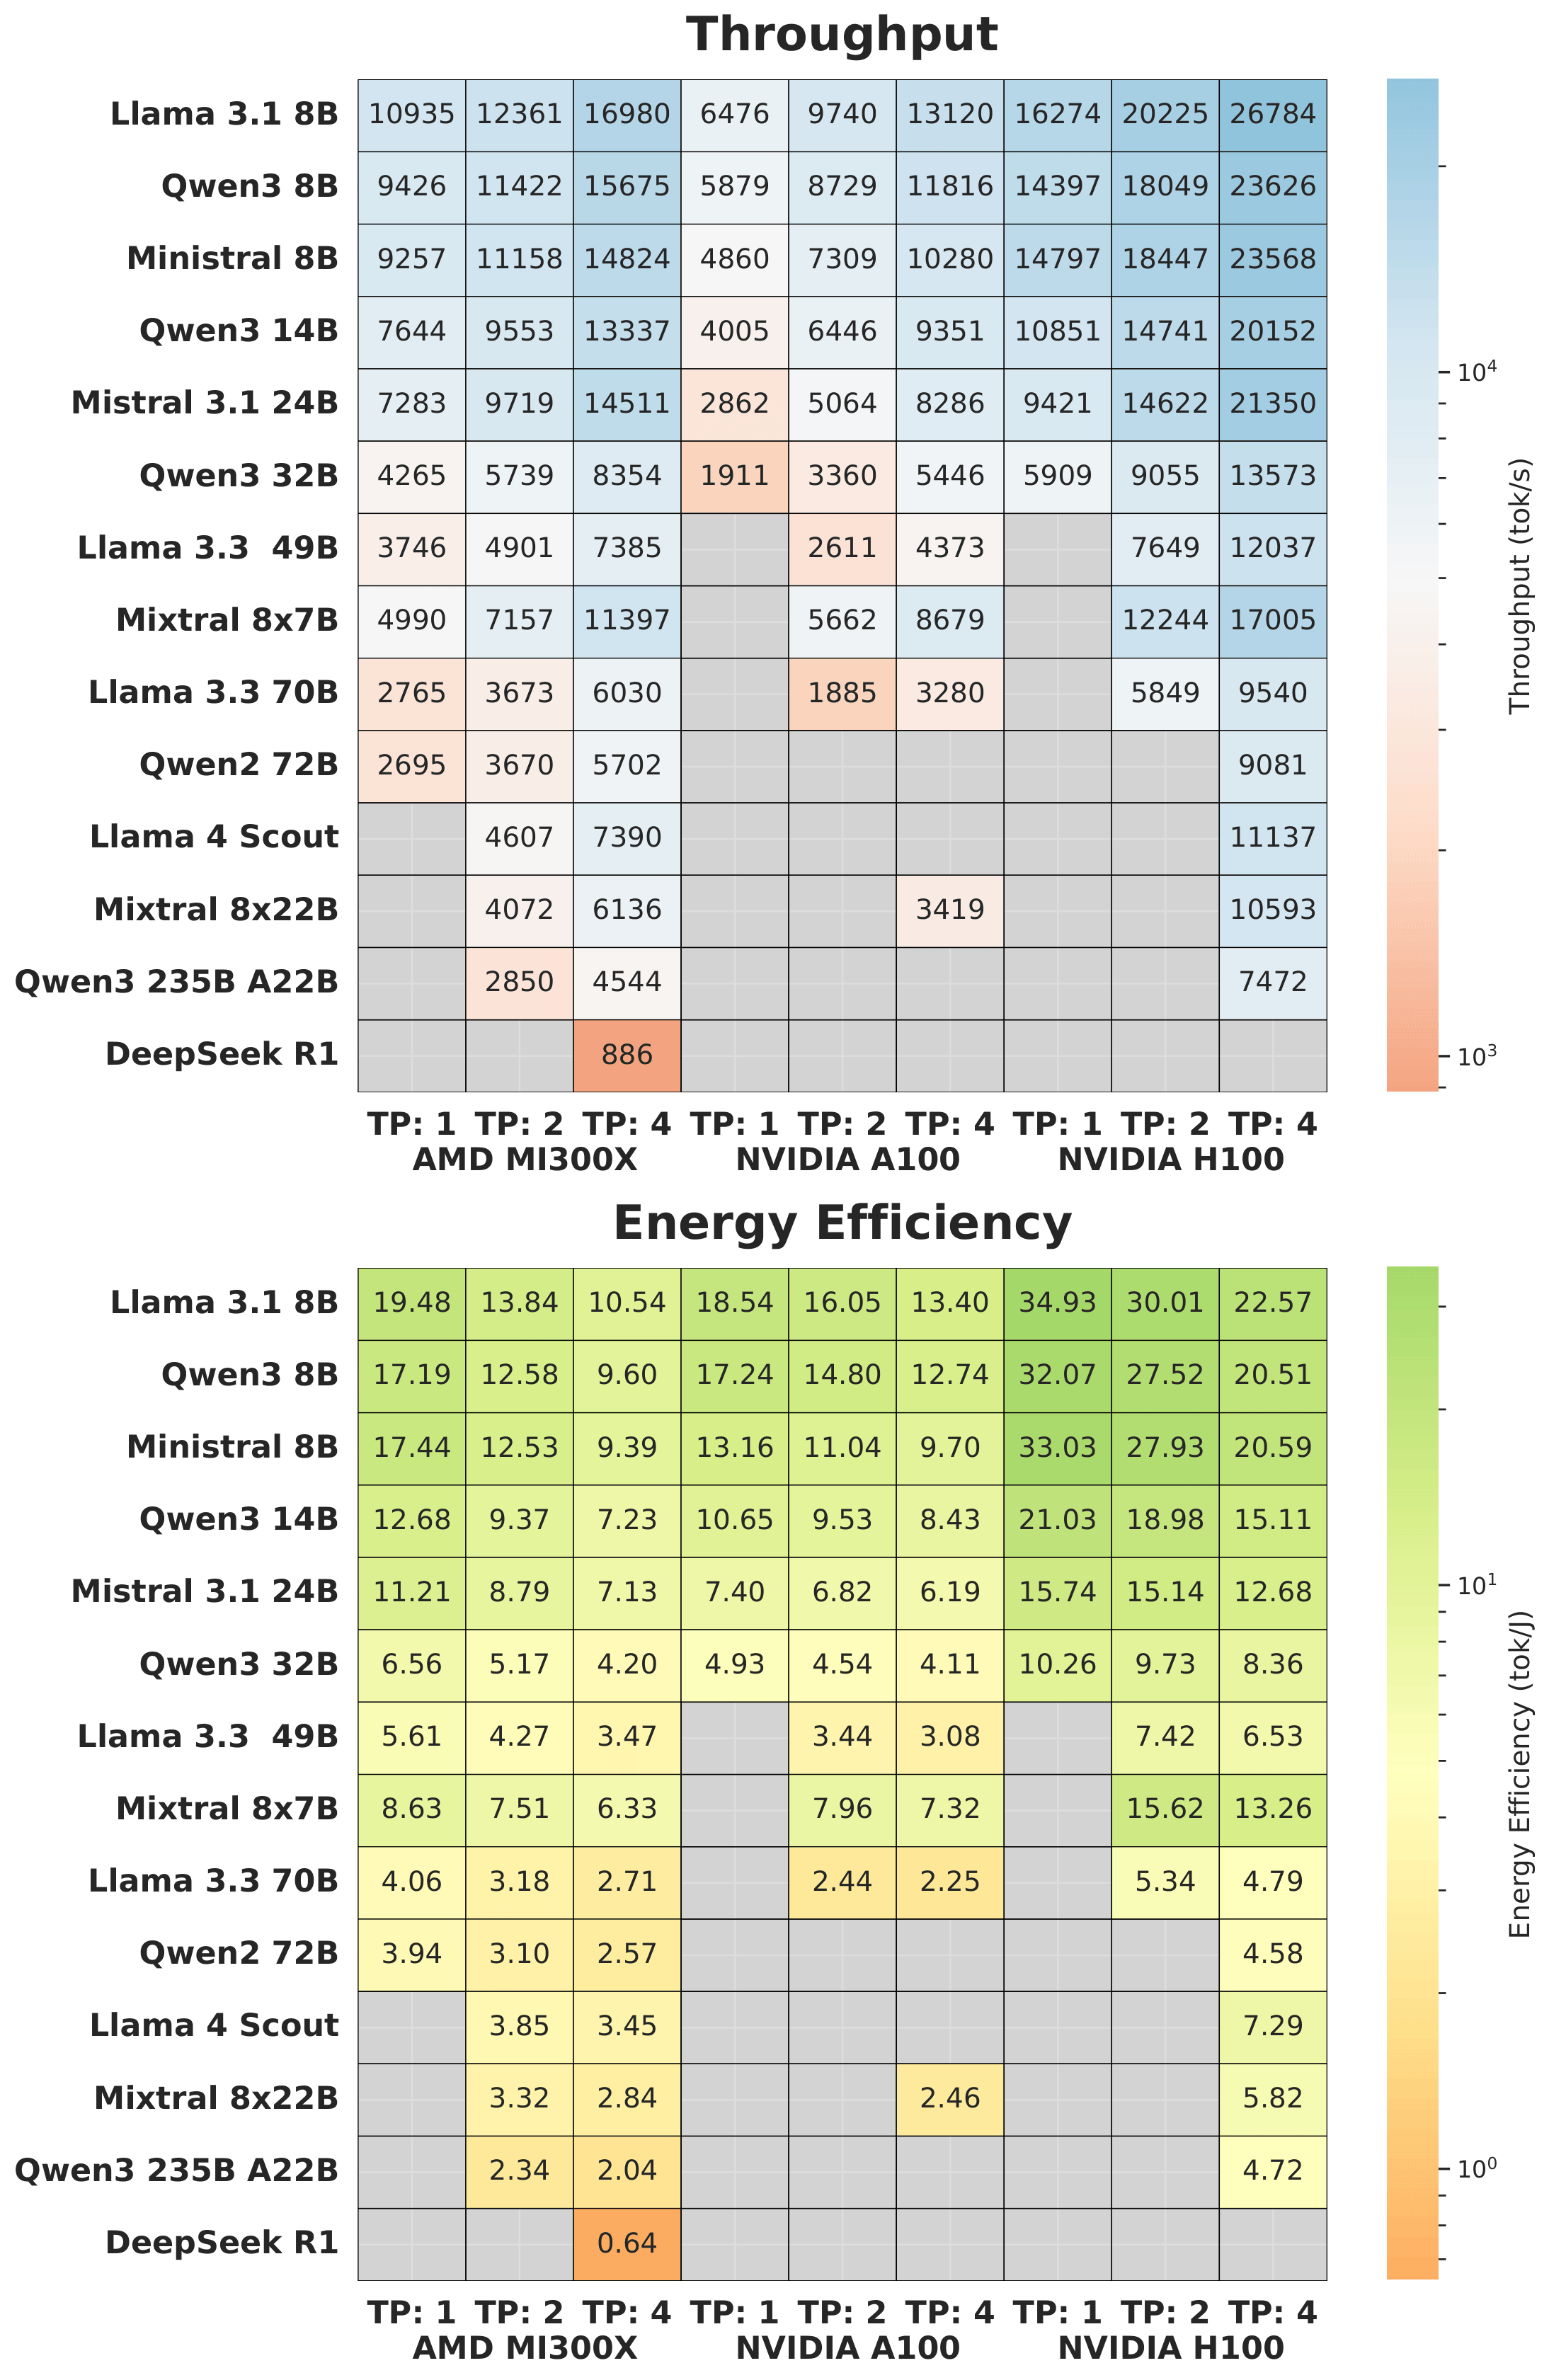
\includegraphics[width=0.9\columnwidth]{figs/heatmap Throughput (toks)_vs_Energy Efficiency (tokJ)_fp8.png}
      \caption{Throughput and energy efficiency heatmap across three multi-GPU nodes (FP8).}
      \tagpdfsetup{alttext={Throughput and energy efficiency heatmap across three multi-GPU nodes (FP8).}}
    \label{fig:heatmapfp8}
\end{figure}


\subsection{Scaling efficiency with 3D Parallelism}
Resource allocation in multi-GPU LLM inference requires balancing memory capacity and computational efficiency when choosing between Tensor and Data Parallelism. As discussed in Section \ref{chap:model:sec:multi}, Tensor Parallelism partitions model weights across GPUs, enabling larger models to run and potentially improving throughput. However, it introduces frequent all-gather operations, which result in synchronization overheads and idle GPU time.

\begin{comment}
\begin{figure}[H]
    \centering
    \includegraphics[width=0.9\columnwidth]{figs/efficiency_lineplot_Throughput per Instance_bfloat16.png}
      \caption{Throughput gain with Tensor Parallelism.}
    \label{fig:tpbars}
\end{figure}
\ref{fig:tpbars} shows how performance improves by increasing the Tensor Parallel size from 1 to 4 in three multi-GPU nodes.
\end{comment}

In our experimental results, we observe that configurations scaled purely with Data Parallelism exhibit an ideal linear scaling.
Instead, configurations that utilize a Tensor Parallel size of 2 or 4 enhance the throughput of the vLLM inference engine; however, display scaling efficiency falls short of the ideal level. Specifically, configurations with Tensor Parallel size 2 yield an average throughput improvement of approximately 33\% (29.9\% on AMD MI300X, 31.4\% on NVIDIA A100, and 37.4\% on NVIDIA H100), while those with Tensor Parallel size 4 achieve about 74\% (73.3\% on AMD MI300X, 74.5\% on NVIDIA A100, and 74.2\% on NVIDIA H100). In terms of scaling efficiency—computed as $\text{Perf}{\text{N-GPUs}} / (N \times \text{Perf}{\text{1-GPU}})$—Tensor Parallel size 2 reaches 65\% efficiency, whereas size 4 reaches 43\%. Compared to data-parallel configurations, which maintain nearly 100\% scaling efficiency, these results indicate that in offline inference scenarios, increasing the number of data-parallel instances is generally more effective for maximizing both throughput and energy efficiency than increasing tensor parallelism.

There are, however, notable exceptions to this general trend. When the model size is large enough that the weights occupy most of the available VRAM, the remaining memory becomes insufficient to support large batch sizes. In such cases, vLLM manages the limitation in two ways: it either dynamically reduces the effective batch size relative to the configured engine setting or, in the event of out-of-memory errors, performs expensive recomputations of segments of the KV matrices. As a result, models that utilize more than 80\% of GPU memory tend to achieve better performance with higher Tensor Parallelism configurations, sometimes even exceeding 100\% scaling efficiency. For instance, Qwen3 32B exhibits higher scaling efficiency with a tensor parallel size of 2 on both NVIDIA A100 and H100 nodes. Similarly, the substantial memory requirements of Llama 3.3 70B make a tensor parallel size of 4 preferable to 2 on the same hardware.

Regarding energy efficiency, a consistent pattern is evident. Data-parallel configurations demonstrate energy efficiency comparable to single-GPU setups, while configurations employing tensor parallelism tend to be less efficient. An exception again occurs for models that use more than 80\% of the available VRAM. As discussed earlier, when hardware remains constant, energy efficiency shows a strong positive correlation with throughput, with correlation coefficients ranging from 0.90 to 0.94. Therefore, optimizing throughput inherently leads to improvements in energy efficiency.

It is also noteworthy that Tensor Parallel configurations generally draw less power on average, as illustrated in \ref{fig:powbars}. However, this reduction in power consumption is insufficient to offset the performance degradation caused by inter-GPU communication overhead. In the specific cases where higher tensor parallelism yields better performance, the lower power usage contributes to energy efficiency gains that exceed the corresponding throughput improvements. This observation further highlights the importance of maintaining sufficient memory capacity for the KV cache.

\begin{figure}[h!]
    \centering
    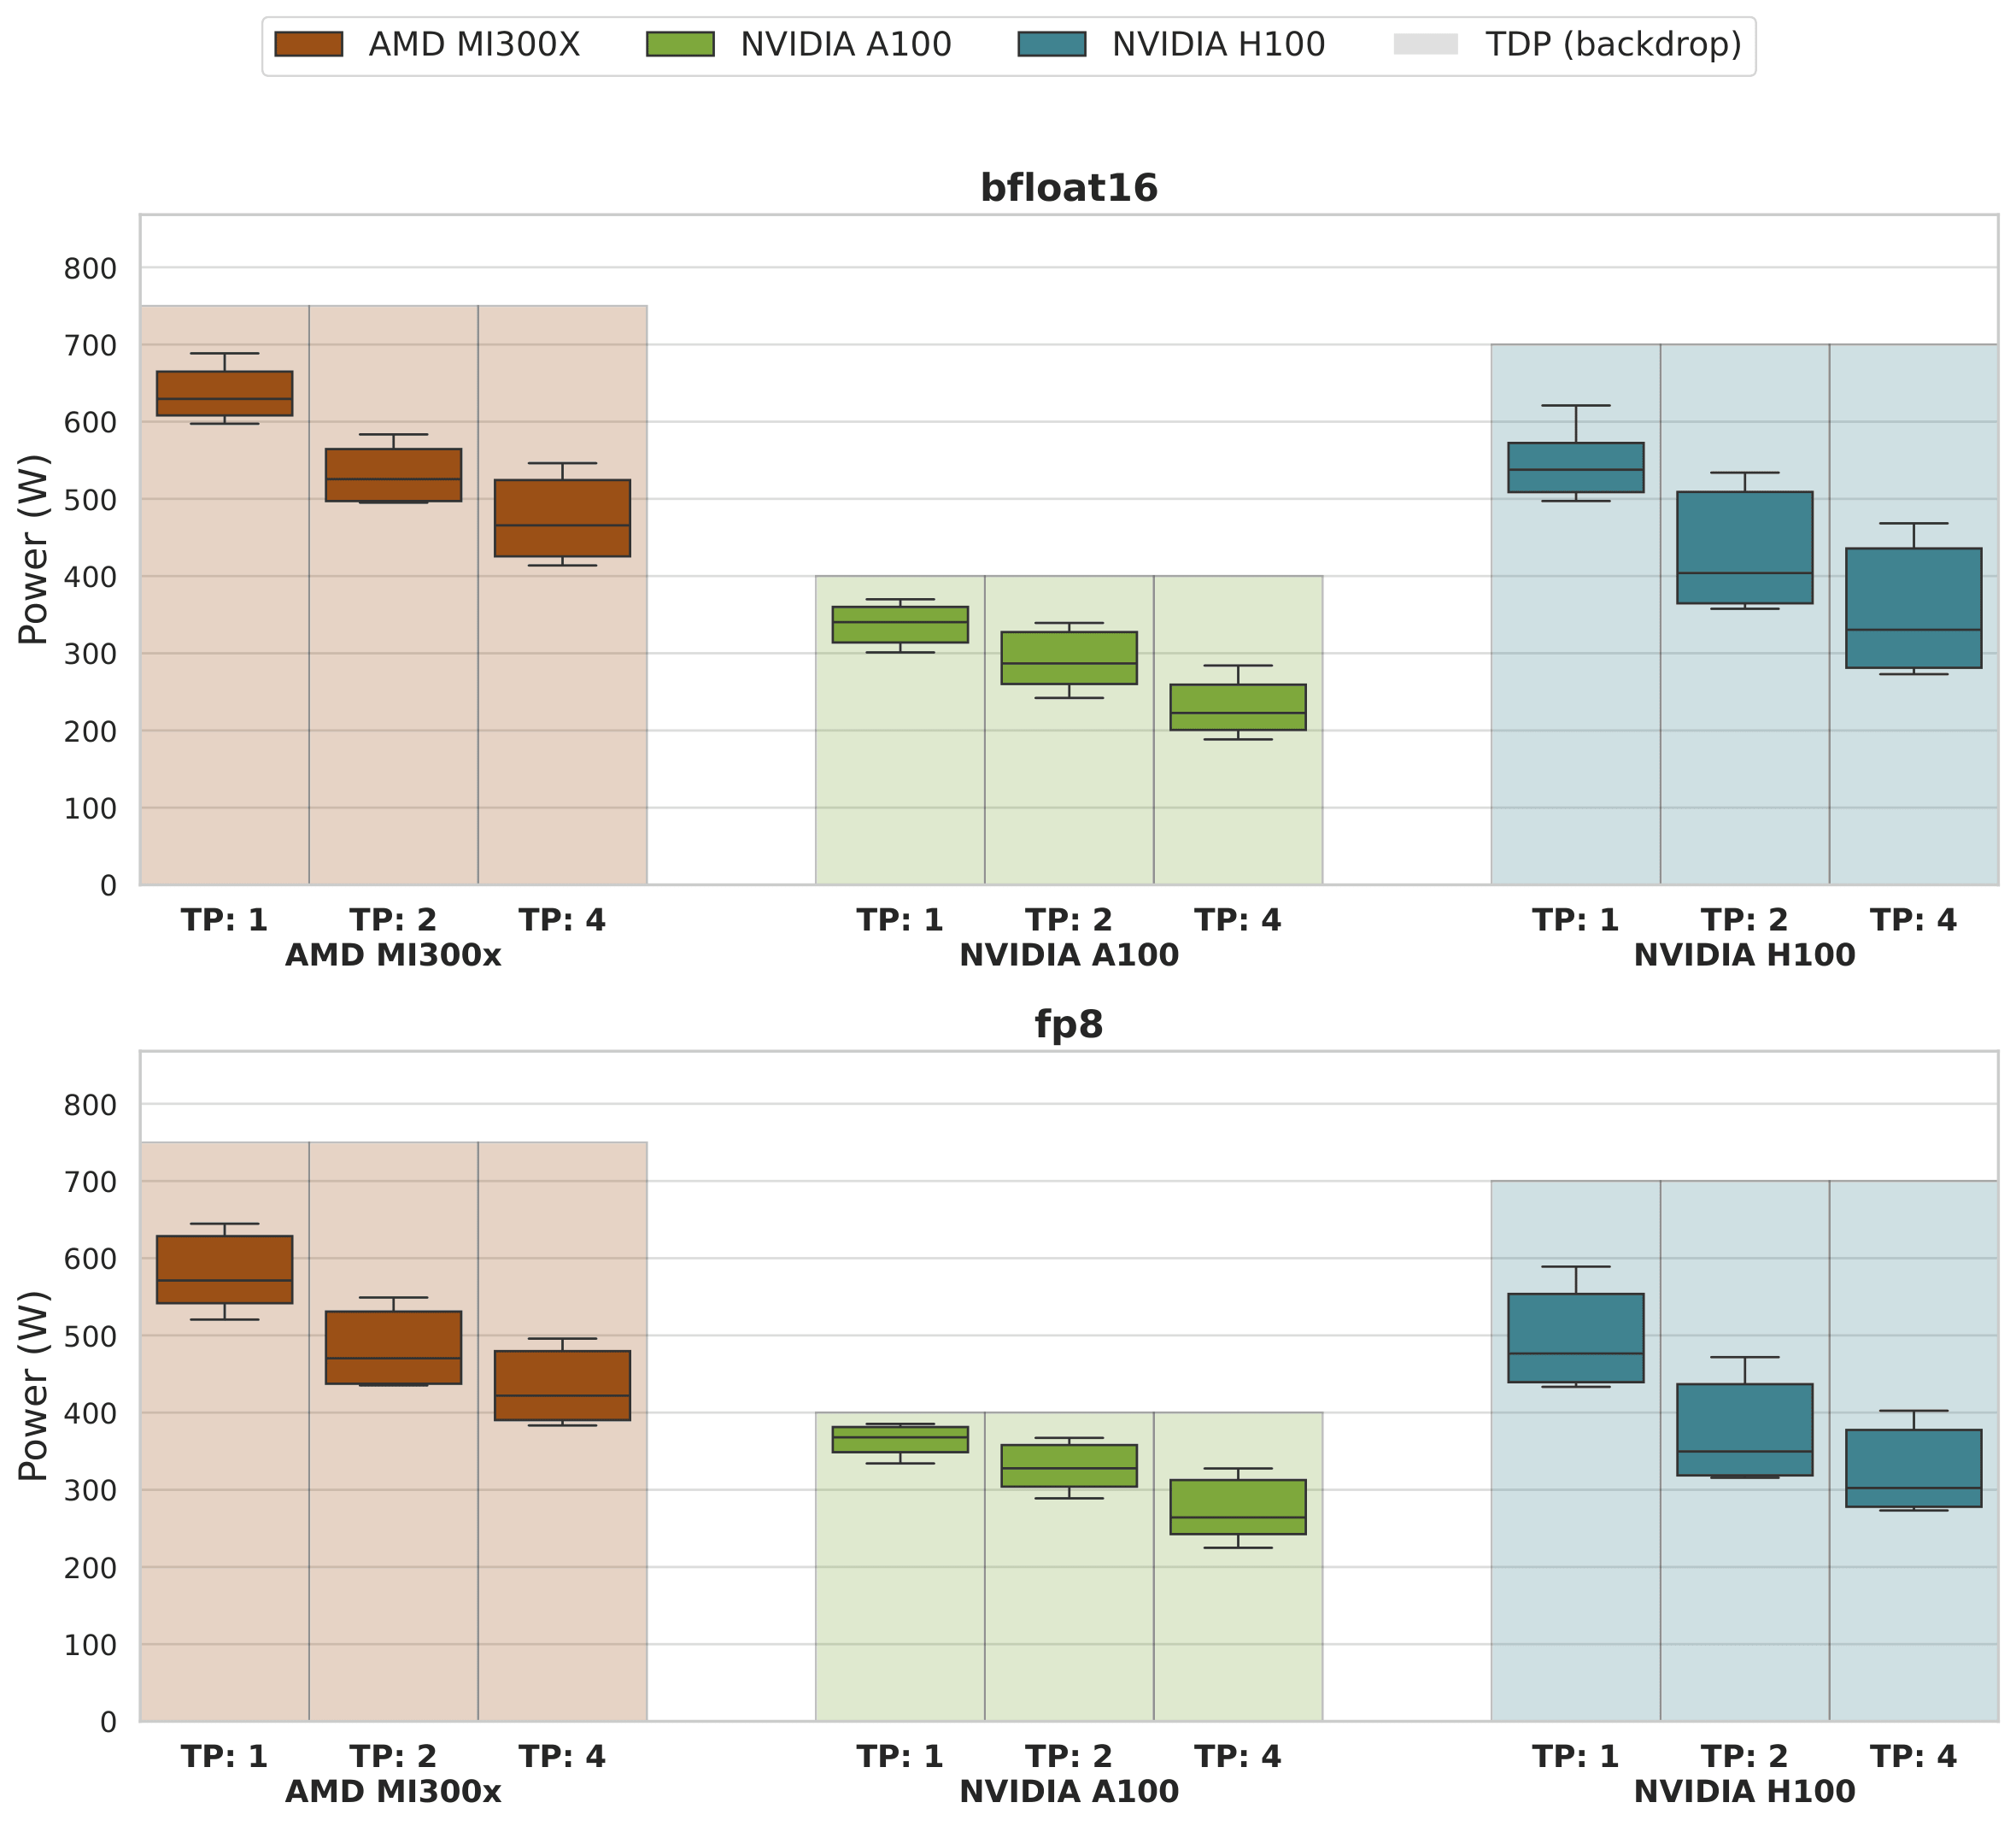
\includegraphics[width=0.95\columnwidth]{figs/efficiency_boxplot_merged_active_power_avg_bfloat16_fp8.png}
    \caption{Power consumption with Tensor Parallelism.}
    \tagpdfsetup{alttext={Power consumption with Tensor Parallelism.}}
    \label{fig:powbars}
\end{figure}

\subsection{Model Size  Scaling}
The second aspect of our analysis investigates how energy efficiency and performance evolve with increasing model size and sparsity. \ref{fig:scaling} presents the trends of four key metrics as the number of parameters increases. The trends across dense models are represented by solid lines, while dashed lines indicate the Mixture-of-Experts (MoE) model.

In Section~\ref{chap:results:sec:single}, we observe that dense models exhibit a linear increase in end-to-end latency and TTFT as model size grows, while throughput and energy efficiency decrease inversely—consistent with the behavior predicted by our performance model, consistently with what was discussed in Section \ref{chap:methods:sec:model}. This trend remains stable even when scaling to multi-GPU configurations with a fixed Tensor Parallel (TP) size.

When comparing different TP/DP configurations, we find that not all metrics scale uniformly under this weak-scaling setting. End-to-end latency and TTFT remain largely constant across TP configurations, whereas throughput and energy efficiency improve in smaller TP setups. Consequently, when considering the best attainable performance across configurations, we observe linear scaling in latency and TTFT, accompanied by an even more pronounced decline in throughput and energy efficiency as model size increases.

A distinct pattern emerges when analyzing Mixture-of-Experts (MoE) models (dashed lines in \ref{fig:scaling}). 
As discussed in \ref{chap:model:sec:moe}, Mixture-of-Experts models activate only a subset of their weights during inference, reducing the number of floating-point operations per forward pass from $2N$ to $2A$, where $N$ is the total number of parameters and $A$ is the number of active parameters. However, their memory load operations depend on the number of experts that are active at each level. In the case of a batch size of 1, loading operations also decrease from $N$ to $A$, while for larger batch sizes, most experts are loaded, resulting in a lower ideal speedup.

When observing experimental data, we can observe that, keeping constant hardware resources, MoE models consistently achieve higher performance and energy efficiency than dense models of comparable size. This demonstrates the effectiveness of the MoE architecture in scaling model parameters and accuracy while maintaining strong computational and energy efficiency. For example, Llama 4 Scout—with 109B total parameters—achieves 17\% higher throughput and 52\% better energy efficiency than the smaller Llama 3 70B on NVIDIA H100, by activating only 17B parameters during inference.
However, due to the impact of memory accesses, these gains are not strictly proportional to the degree of sparsity. On both NVIDIA H100 and AMD MI300X, Llama 4 Scout underperforms relative to Llama 3 Nemotron Super (49B), despite activating only 22B parameters.

\begin{figure}[h!]
    \centering
    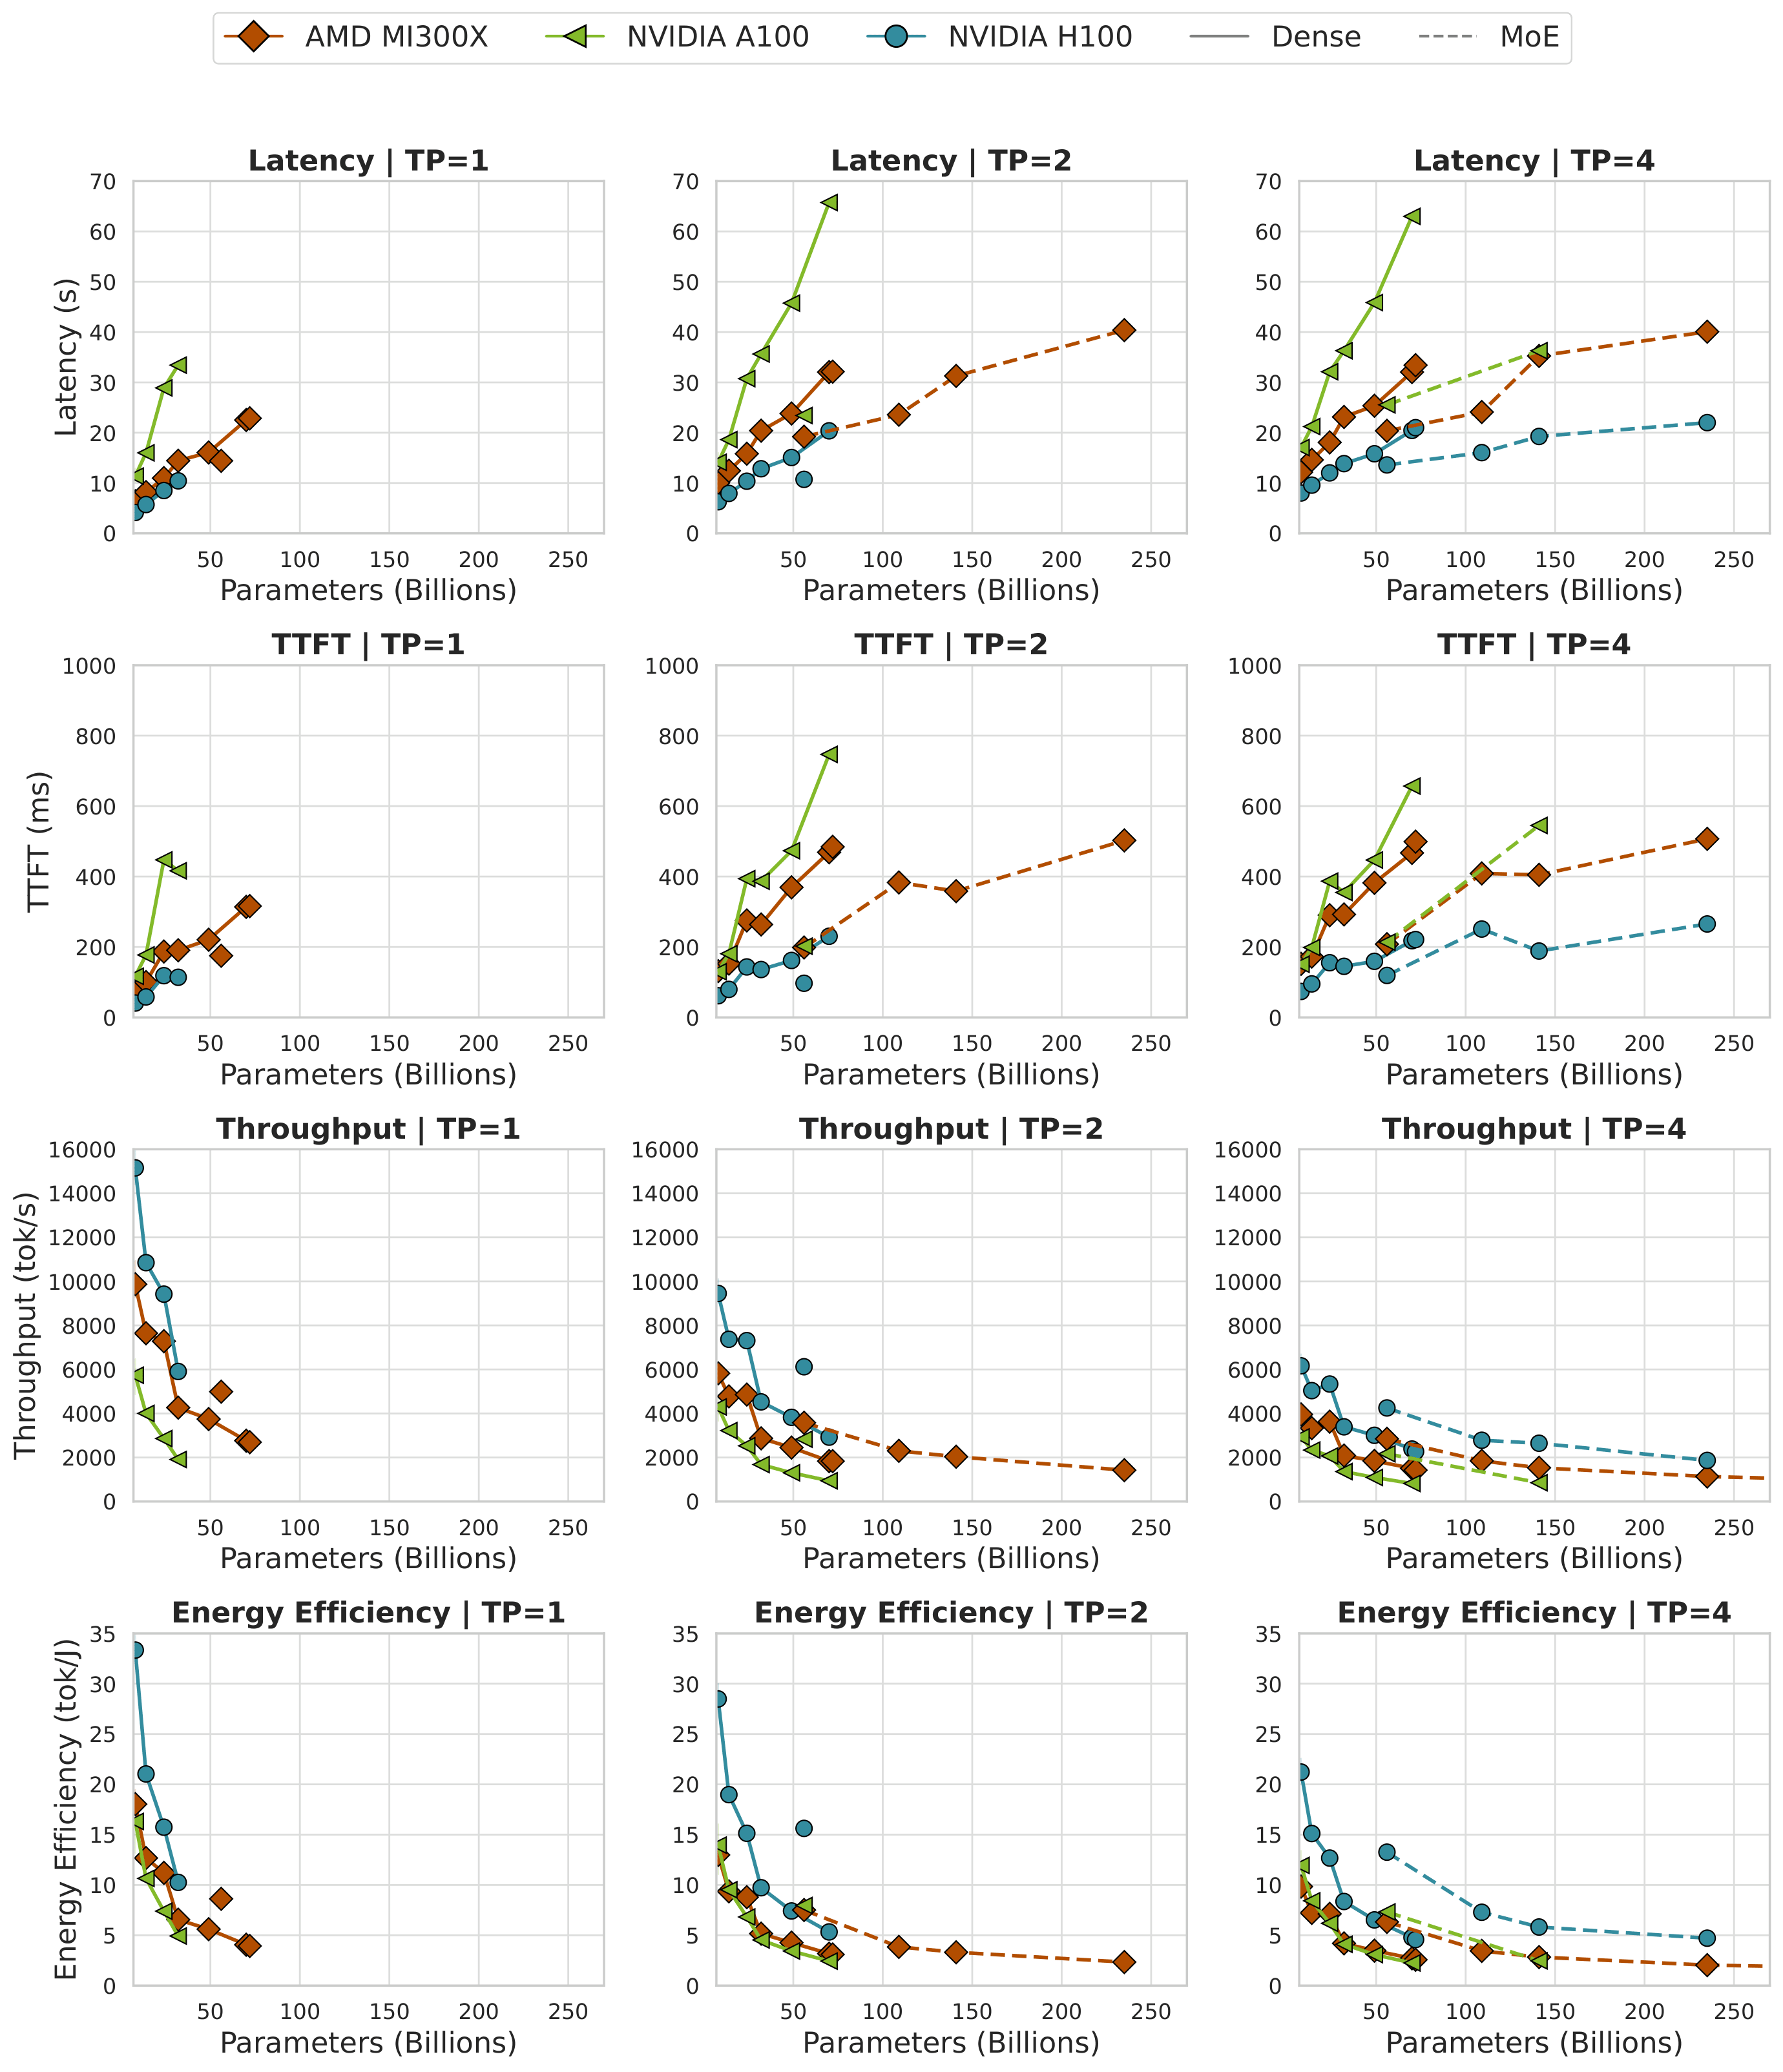
\includegraphics[width=\columnwidth]{figs/Combined_Metrics_NoBest.png}
      \caption{Scaling of performance metrics with model size.}
      \tagpdfsetup{alttext={Scaling of performance metrics with model size.}}
    \label{fig:scaling}
\end{figure}

\subsection{Tensor and Expert Parallelism}
In Section \ref{chap:background:sec:serving}, we introduced Expert Parallelism as an alternative approach to parallelizing inference in Mixture-of-Experts (MoE) models.
To evaluate its performance, we conduct a series of experiments comparing Tensor Parallelism and Expert Parallelism across four sparse large language models (LLMs). Each model is tested on both four NVIDIA H100 GPUs and four AMD MI300X GPUs, using both parallelization strategies and a range of batch sizes.

\begin{figure}[h!]
\centering
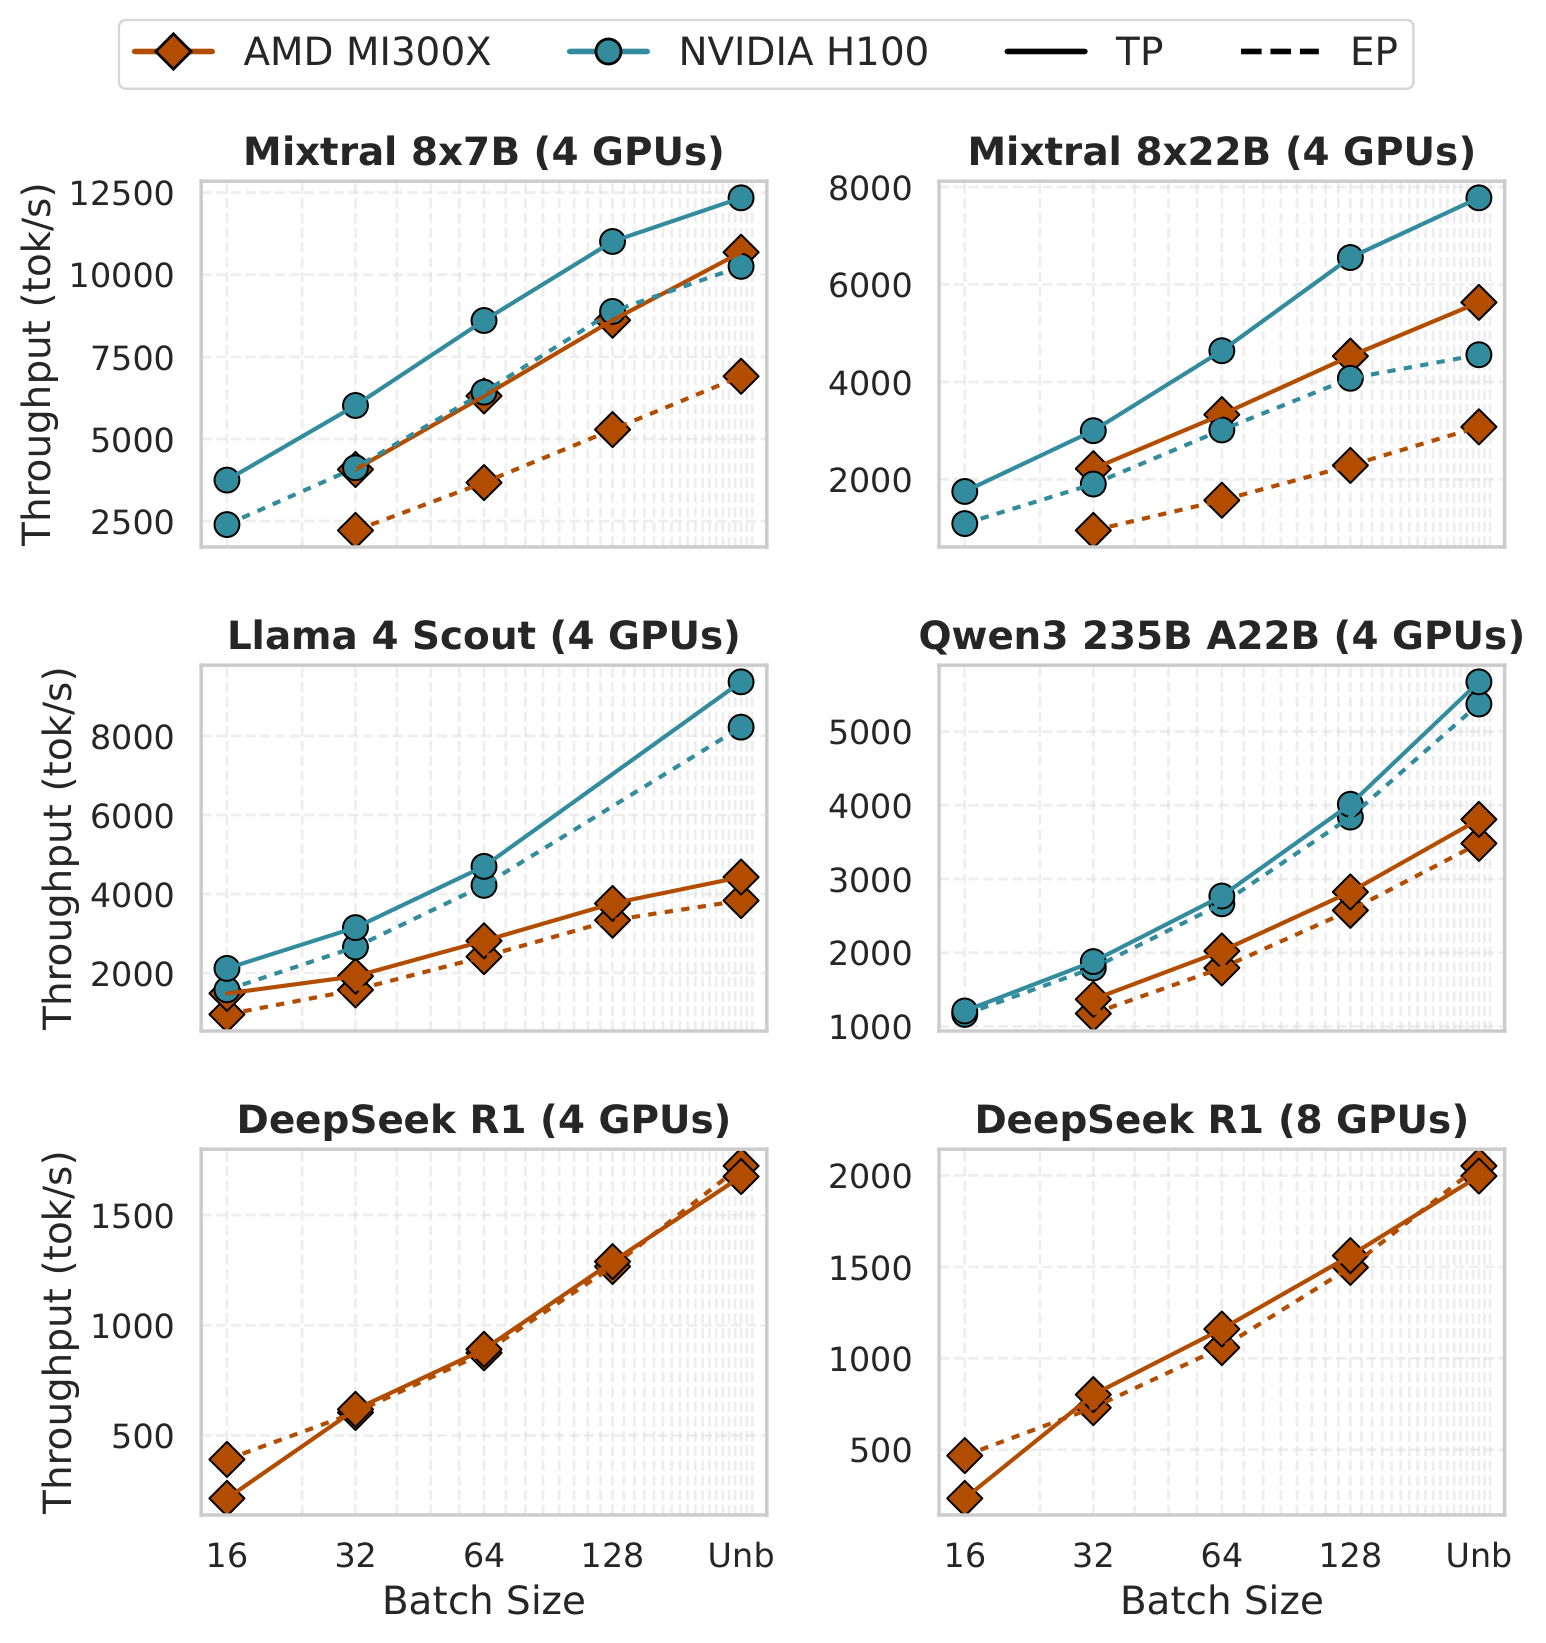
\includegraphics[width=0.75\columnwidth]{figs/combined_ep_tp.png}
\caption{Throughput using Tensor and Expert Parallelism.}
\tagpdfsetup{alttext={Throughput using Tensor and Expert Parallelism.}}
\label{fig:ep}
\end{figure}

At a first-level analysis, the results show that Tensor Parallelism consistently outperforms Expert Parallelism across all models, batch sizes, and hardware configurations—with one notable exception, which is discussed later.

A closer examination of model architectures reveals that the number of experts is a key factor driving this performance gap. Mixtral 8x22B, which employs eight experts, exhibits the largest advantage for Tensor Parallelism, achieving 61\% higher throughput on the H100 and up to 2.7 $\times$ higher throughput on the MI300X. For Llama 4 Scout (16 experts), Tensor Parallelism achieves 6\% higher throughput on the MI300X and 34\% higher throughput on the H100. Qwen3, with 128 experts, shows smaller improvements (16\% on MI300X and 4\% on H100). DeepSeek R1, however, deviates from this pattern due to its unique configuration—256 rooted experts plus one shared expert—which enables Expert Parallelism to match or exceed Tensor Parallelism at smaller batch sizes. At a batch size of 16, it achieves 82\% higher throughput with four GPUs and 100\% higher throughput with eight GPUs. As the batch size increases, this advantage diminishes, and both methods converge to similar performance levels.

The energy efficiency results largely reflect the throughput trends. Tensor Parallelism generally proves more energy-efficient, particularly for models with fewer experts. For instance, Mixtral 8x22B achieves twice the efficiency on the MI300X and a 60\% improvement on the H100, while Llama 4 Scout exhibits comparable gains. Qwen3 again shows marginal improvements (18\% on MI300X and 2\% on H100). DeepSeek R1 remains the exception: Expert Parallelism is more efficient at batch sizes of 16 or smaller, but Tensor Parallelism becomes more efficient as the batch size grows.


\subsection{GPU Model Comparison}
\ref{fig:heatmapbf16} and \ref{fig:heatmapfp8} report the throughput and energy efficiency of all the experimental results conducted with the three multi-GPU nodes in bfloat16 and FP8 precision, respectively.

Consistent with the findings presented in Section \ref{chap:results:sec:single}, the NVIDIA H100 achieves the highest throughput among all tested GPUs, in both bfloat16 and FP8 precisions. It is followed by the AMD MI300X, which consistently outperforms the NVIDIA A100. The performance gap between NVIDIA Hopper and AMD CDNA3 architectures, relative to NVIDIA Ampere, becomes more pronounced under FP8 quantization, as the newer architectures incorporate dedicated FP8 functional units that support W8A8 quantization, in contrast to W8A16 on Ampere.

In terms of energy efficiency, the results vary depending on the precision and model size. With bfloat16 precision, the NVIDIA A100 demonstrates higher efficiency than the AMD MI300X for models with fewer than 32B active parameters. However, when using FP8 quantization, the MI300X consistently exhibits superior efficiency. Across all configurations, the NVIDIA H100 maintains the highest overall efficiency at both precisions.

Memory capacity also plays a crucial role in determining performance. While both NVIDIA GPUs provide 80 GB of HBM memory, the AMD MI300X offers 192 GB, yielding two major advantages: it can accommodate larger models and requires smaller tensor parallel sizes for equivalent workloads. As discussed earlier, Tensor Parallelism introduces frequent all-gather operations that hinder performance, making lower tensor parallel sizes desirable.

When comparing performance under a fixed GPU budget (e.g., four GPUs), the MI300X often achieves higher throughput due to its larger memory capacity. This enables it to operate in pure data-parallel mode, avoiding the communication overheads inherent to high tensor parallel sizes on NVIDIA systems. For instance, with Llama 3.3 70B in bfloat16 precision, the MI300X achieves approximately 2017 tokens per second per GPU with a tensor parallel size of 1, resulting in a total throughput of 8068 tokens per second across four GPUs. In contrast, the NVIDIA H100 reaches 7634 tokens/s under the same configuration but requires a tensor parallel size of 4. A similar pattern emerges for Qwen2 72B in bfloat16 precision.
